\section{Labels}\label{sec:labels}

\subsection{Overview}


Concurrent programs are a mix of control constructs ($\cseq,\parallel,+,\dots$)
and atomic actions $a$ that modify \emph{program state} $s$.
This is all that is visible to the programmer.



Our denotational UTP semantics
is inspired by that done for UTPP\cite{DBLP:conf/icfem/WoodcockH02},
itself based on a UTP theory of \emph{action systems}.
First, we add a new state component, not visible in the program text,
which is a set of labels ($ls$).
These labels are used to orchestrate the flow of control.
Given an atomic action $a$ that only knows about program state $s$,
we use notation $\catom a$ to describe a lifted version
of $a$ that takes account of the contents of the label-set $ls$.
In effect a lifted atomic state action is disabled until
a particular label is present in that set.
A disabled action does not modify the state any way
and simply monitors the label-set.
Once an action observes the presence/arrival of its label,
it then becomes active.
An active lifted action $\catom a$ atomically modifies the extended state as follows:
\begin{itemize}
  \item It makes the changes to $s$ as determined by its underlying action $a$.
  \item It removes the enabling label from the label-set.
  \item It adds in appropriate ``continuation'' labels to $ls$.
\end{itemize}
In \cite{DBLP:conf/icfem/WoodcockH02},
the language syntax required explicit (starting) labels
for every atomic state change action,
and these are used as lifted action enablers.
The continuation labels were taken to the the enabling labels
of whatever other actions occurred immediately after, in the program.
This means that the resulting semantics is not compositional.

The approach we adopt is to adopt the notion of \emph{label generators}
to create the labels, so ensuring they are unique,
but in such a way as make the generation a compositional process.
In addition we explicitly associate two labels with every program construct:
one that marks the entry into the construct,
and another that indicates the exit.
In our UTP theory we will introduce two static observation variables,
$in$ and $out$ to record respectively the entry and exit labels
for a given construct.


\subsection{Label Generation}

We want to have a way to associate unique labels
with every atomic action, including those added to manage flow of control,
in a compositional manner.
We start by assuming that we have types for labels,
and label generators:
\RLEQNS{
   l &\in& Lbl
\\ g &\in& Gen
}
We have two distinct things we can do with label generators:
\begin{enumerate}
  \item
   Use it then generate a label,
   in which case we also need to get a transformed generator
   that is guaranteed to never produce the label just generated.
   \RLEQNS{
     new &:&  Gen \fun (Lbl \times Gen)
     & \elabel{new-sig}
   }
  \item
   Split generators into two new generators,
   each of which will produce disjoint sets of labels.
   \RLEQNS{
     split &:& Gen \fun (Gen \times Gen)
     & \elabel{split-sig}
   }
\end{enumerate}
Given $new$ and $split$ above, we can defined a function $labs$ that
returns all the labels produced by a generator,
and express our label uniqueness guarantees.
Assuming that $ (l,g') = new(g)$ and $(g_1,g_2) = split(g)$
we get:
\RLEQNS{
   labs &:& Gen \fun \power Lbl & \elabel{labs-sig}
\\ labs(g)
   &\defs&
   \setof l \cup labs(g')
   \cup
   labs(g_1) \cup labs(g_2) &\ecite{labs-def}
\\ l &\notin& labs(g') &\ecite{new-disj}
\\ labs(g_1) \cap labs(g_2) &=&  \emptyset & \ecite{split-disj}
}

Given the notion of label generators as just described,
we are faced with two problems.
The first is that the notation is quite clumsy:
For example in the semantics to be presented below,
we will need the following generator expression:
$
\pi_2(new(\pi_2(new(\pi_2(split(g))))))
$,
where $\pi_i$ projects out the $i$th element of a pair.
The second is that our definitions above are axiomatic,
and we need to demonstrate some form of model that satisfies
the above laws (\ecite{new-disj},\ecite{split-disj}).
Ideally this should also avoid some sort of global check for uniqueness,
to ensure compositionality of the resulting semantics.

Fortunately,
it turns out there is a shorthand notation that dramatically shortens
generator and label expressions,
while also providing a compositional model that satisfies the laws above.

\subsubsection{Generator Notation}

The idea is to realise that we really have four functions of interest:
\RLEQNS{
   \pi_1 \circ new &:& Gen \fun Lbl
\\ \pi_2 \circ new &:& Gen \fun Gen
\\ \pi_1 \circ split &:& Gen \fun Gen
\\ \pi_2 \circ split &:& Gen \fun Gen
}
For the first one, we shall define a prefix operator $\ell : Gen \fun Lbl$
and render its generator argument as a subscript:
\RLEQNS{
  \ell_g &\defs& \pi_1(new(g)) & \elabel{ell-def}
}

For the other three, we turn them into single-character postfix operators,
themselves being rendered as subscripts:
\RLEQNS{
   \g{:} &\defs& \pi_2 \circ new & \elabel{new-:-def}
\\ \g1   &\defs& \pi_1 \circ split & \elabel{split-1-def}
\\ \g2   &\defs& \pi_2 \circ split & \elabel{split-2-def}
}
We then introduce a notation of generator and label expressions
with the following syntax:
\RLEQNS{
   G \in Gen &::=&  g     & \mbox{the ``root'' generator}
\\           &\mid& G_{:} & \mbox{resulting generator after label produced}
\\           &\mid& G_1   & \mbox{first generator after generator split}
\\           &\mid& G_2   & \mbox{second generator after generator split}
\\ L \in Lbl &::=& \ell_G & \mbox{label produced by generator}
}
Note that our generator expression language has only one variable, $g$,
which denotes the ``root'' generator.
We say the  ``root'' generator because this notion is local to a
particular context, and we can relativise things by replacing $g$
by an appropriate $G$ expression.
We can now revisit our definition of $labs$ and our disjointness rules
with the new notation:
\RLEQNS{
   labs &:& Gen \fun \power Lbl
\\ labs(G) &=& \setof{\ell_G} \cup labs(G_{:}) \cup labs(G_1) \cup labs(G_2)
  &\elabel{labs-def}
\\ \ell_G &\notin& labs(G_{:})
   &\elabel{new-disj}
\\ \emptyset &=& labs(G_1) \cap labs(G_2)
  &\elabel{split-disj}
}
The our complicated example shown earlier:
\[
\pi_2(new(\pi_2(new(\pi_2(split(g))))))
\]
now reduces to
\[
  \g{2::}
\]

We can also introduce a graphical way to visualise
generators that proves useful as a way to understand
the semantic definitions that occur later on,
as shown in Fig. \ref{fig:new-and-split}
\begin{figure}%
  \centering
  \parbox{1.2in}{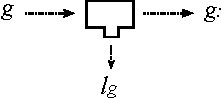
\includegraphics{images/new-label}}%
  \qquad\qquad
  \begin{minipage}{1.2in}%
    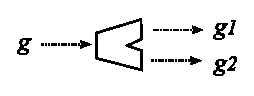
\includegraphics{images/split-gen}
  \end{minipage}%
  \caption{Graphical renderings of $new$ (left) and $split$ (right)}%
  \label{fig:new-and-split}%
\end{figure}



\subsubsection{Model for $new$ and $split$}

The conceptually simplest model of such generators
is one where labels produced are simply the strings of $:$, $1$ and $2$
that designate how the generator was produced from the original root.
For full clarity we show the model here using the full notation.
Both generators and labels are now represented as sequences of the three symbols
$:$, $1$ and $2$.
\RLEQNS{
  s \in LblSym &=& \setof{\texttt{:},\texttt{1},\texttt{2}}
\\ g \in GenSym &=& LblSym^*
\\ l \in Label &=& LblSym^*
\\ new(g) &\defs&  (g,g \cat \seqof{\texttt{:}})
\\ split(g) &\defs&  (g \cat \seqof{\texttt{1}},g \cat \seqof{\texttt{2}})
}
With this model we also get the following law:
For any generator expression $G$,
the following four sets are mutually disjoint:
\[
  \setof{\ell_G}
  \quad
  labs(G_{:})
  \quad
  labs(G_1)
  \quad
  labs(G_2)
  \qquad
  \elabel{labs-fully-disjoint}
\]
This is stronger than we require, but this is not a problem.
We also get two very significant benefits from this model/notation:
\begin{enumerate}
  \item
    It is very easy to decide if two generator expressions produce
    disjoint labels.
    This occurs if and only if neither of the sequences of postfix operators
    involved are a prefix of the other.
    Or put differently, a generator's labels are a subset of another's
    iff its postfix sequence extends that of the other generator:
    \RLEQNS{
       labs(\g{\rho}) \subseteq labs(\g{\varrho}) &\equiv& \varrho \leq \rho
       & \elabel{prefix-lab-subset}
    }
    where $\leq$ is the sequence prefix relation.
  \item
    We refer to $g$ as the ``root'' in double quotes,
    because $g$ is not privileged in any way.
    If we substitute a different expression $G$ for $g$
    in the semantics of a construct,
    the behaviour is unchanged.
    In effect $g$ is like a ``base address'',
    with all the labels generated from $g$ being relative to it,
    and replacing $g$ by $G$ simply relocates it and the labels it generates.
    This is the basic mechanism used to construct the semantics
    of all the composite constructs in the language.
\end{enumerate}


\subsection{Label-Set Invariants}


We want to distinguish between disjointness only:
\[ \{ in | g | out \} \]
from disjointness with label-set exclusion:
\[ [ in | g | out ] \]

We want to be able to specify that certain combinations
of labels should never appear simultaneously
in the global label set ($ls$).
We do this by defining a label-set invariant $I$
which has alphabet $ls,in,out,g$.

We start by defining a general abstract way of specifying
sets with valid combinations
of values drawn from a parameter type $\tau$.
\RLEQNS{
   i \in I_\tau &::=& \tau   &  \mbox{can contain this value}
\\ &\mid& \otimes(i,\ldots,i) & \mbox{at most one of these allowed to contain}
\\ &\mid& \cup (i,\ldots,i) & \mbox{any of these allowed to contain}
}

We define what it means for an atomic action invocation
to satisfy an invariant parameterised on the label type ($Lbl$).
\RLEQNS{
  ls \textbf{ lsat } I \land A(E|a|N) &\implies& ls' \textbf{ lsat } I
}
We can re-formulate this as a following equivalent test:
\RLEQNS{
   A(E|a|N) \textbf{ sat } I_{Lbl}
   &\defs&
   E \textbf{ lsat } I_{Lbl} \land N \textbf{ lsat } I_{Lbl}
}
In effect we identify the occurrences of labels within this $I$-structure,
and then check the multiplicity constraints:
\RLEQNS{
   L \textbf{ lsat } I_{Lbl} &\defs& res=ok
\\ \textbf{where} && (res,\_) = occChk (occ_L I_{Lbl})
}
The $occ$ function takes a set $L$ of $\tau$ and an $I_\tau$ and returns a $I_\Bool$
that records if the corresponding element of $\tau$ is present in $L$.
\RLEQNS{
   occ &:& \power \tau \fun I_\tau \fun I_\Bool
\\ occ_L~\ell &\defs& \ell \in L
\\ occ_L~\otimes(i_1,\ldots,i_n)
   &\defs&
   \otimes(occ_L~i_1,\ldots,occ_L~i_n)
\\ occ_L~\cup(i_1,\ldots,i_n)
   &\defs&
   \cup(occ_L~i_1,\ldots,occ_L~i_n)
}
The $occChk$ function pattern matches across the boolean values to see if
constraints are satisfied.
The first component of the result is an overall ok/fail indicator,
while the second boolean component indicates if values are present
in any component.
\RLEQNS{
   occChk &:& I_\Bool \fun (\setof{ok,fail}\times \Bool)
\\ occChk(b) &\defs& (ok,b)
\\ occChk(\cup(i_1,\ldots,i_n))
   &\defs&
   (fail,\_),
   \textbf{ if }\exists j @ occChk(i_j) = (fail,\_)
\\ && (ok,b_1 \lor \dots \lor b_n),
   \textbf{ if }\forall j @ occChk(i_j) = (ok,b_j)
\\ occChk(\otimes(i_1,\ldots,i_n))
   &\defs&
   (fail,\_),
   \textbf{ if }\exists j @ occChk(i_j) = (fail,\_)
\\&& (fail,\_) \mbox{ if more than one $(ok,true)$}
\\&& (ok,false) \mbox{ if all are $(ok,false)$}
\\&& (ok,true) \mbox{ if  exactly one $(ok,true)$}
}
We note, as a consequence of the above definitions, that
\RLEQNS{
  \emptyset &  \textbf{lsat} &  I & \elabel{emp-lsat-I}
}
for any label-set invariant $I$.

We introduce a shorthand for invariants illustrated as follows.
\RLEQNS{
  ~ [ a,b,c | d,e | f ]
   &=&
   ls \textbf{ lsat } \otimes(\cup(a,b,c),\cup(d,e),f)
\\ ~[ a | (b|c),(d|e) | f ]
  &=&
  ls \textbf{ lsat } \otimes(a,\cup(\otimes(b,c),\otimes(d,e)),f)
}
In effect we make the involvement of $ls$ implicit,
and use bar ($|$) and comma ($,$) to replace $\otimes$ and $\cup$ respectively.
We also have a shorthand that just denotes
the non-intersecting nature of the arguments.
E.g.,
$\setof{A|B|C}$ asserts that $A$, $B$ and $C$ are mutually disjoint,
without any reference to $ls$ or any other set.

\subsubsection{Invariant Examples}

The following examples show how various instances of $ls \textbf{ lsat } I$
get expanded:
\RLEQNS{
   ~[in|out]
   &=&
   \setof{in} \cap \setof{out} = \emptyset
\\ &\land&
  \setof{in} \subseteq ls \implies \setof{out}\cap ls = \emptyset
\\ &\land&
  \setof{out} \subseteq ls \implies \setof{in}\cap ls = \emptyset
\\
\\ ~[in|\ell|out]
   &=&
   \setof{in} \cap \setof{\ell,out} = \emptyset
\\ &\land&
   \setof{\ell} \cap \setof{in,out} = \emptyset
\\ &\land&
   \setof{out} \cap \setof{in,\ell} = \emptyset
\\ &\land&
  \setof{in} \subseteq ls \implies \setof{\ell,out}\cap ls = \emptyset
\\ &\land&
  \setof{\ell} \subseteq ls \implies \setof{in,out}\cap ls = \emptyset
\\ &\land&
  \setof{out} \subseteq ls \implies \setof{in,\ell}\cap ls = \emptyset
\\
\\ ~[ a | (b|c),(d|e) | f ]
   &=&
   \setof{a} \cap \setof{b,c,d,e,f} = \emptyset
\\ &\land&
   \setof{b,c,d,e} \cap \setof{a,f} = \emptyset
\\ &\land&
   \setof{f} \cap \setof{a,b,c,d} = \emptyset
\\ &\land&
  \setof{a} \subseteq ls \implies \setof{b,c,d,e,f}\cap ls = \emptyset
\\ &\land&
  \setof{b,c,d,e} \subseteq ls \implies \setof{a,f}\cap ls = \emptyset
\\ &\land&
  \setof{f} \subseteq ls \implies \setof{a,b,c,d,e}\cap ls = \emptyset
\\ &\land&
   \setof{b} \cap \setof{c} = \emptyset
\\ &\land&
   \setof{d} \cap \setof{e} = \emptyset
\\ &\land&
  \setof{b} \subseteq ls \implies \setof{c}\cap ls = \emptyset
\\ &\land&
  \setof{c} \subseteq ls \implies \setof{b}\cap ls = \emptyset
\\ &\land&
  \setof{d} \subseteq ls \implies \setof{e}\cap ls = \emptyset
\\ &\land&
  \setof{e} \subseteq ls \implies \setof{d}\cap ls = \emptyset
}
Here one of $b$ or $c$ may occur in $ls$ along with one of  $d$ or $e$.
In this theory,
we use the label generators to ensure that the disjointness
conditions of the invariants are always true, by construction.

\subsubsection{Notation}

\RLEQNS{
   ls(\ell) &\defs& \ell \in ls
\\ ls(L) &\defs& L \subseteq ls
\\ ls(\B\ell) &\defs& \ell \notin ls
\\ ls(\B L) &\defs& L \cap ls = \emptyset
}
